% This file was created by matplotlib2tikz v0.6.18.
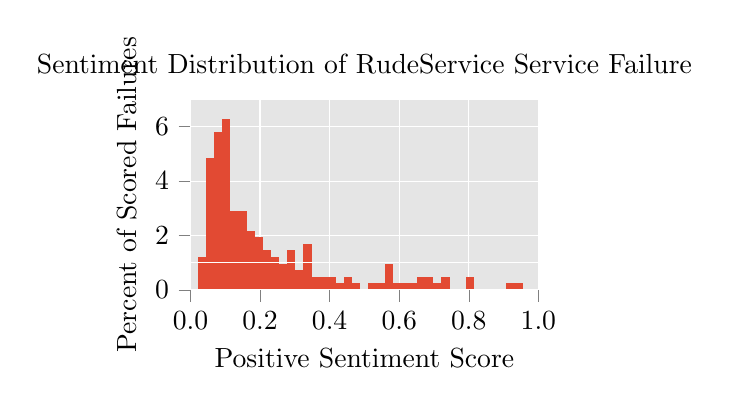
\begin{tikzpicture}

\definecolor{color0}{rgb}{0.886274509803922,0.290196078431373,0.2}

\begin{axis}[
axis background/.style={fill=white!89.80392156862746!black},
axis line style={white},
height=4cm,
tick align=outside,
tick pos=left,
title={Sentiment Distribution of RudeService Service Failure},
width=6cm,
x grid style={white},
xlabel={Positive Sentiment Score},
xmajorgrids,
xmin=0, xmax=1,
xtick={0,0.2,0.4,0.6,0.8,1},
xticklabels={0.0,0.2,0.4,0.6,0.8,1.0},
y grid style={white},
ylabel={Percent of Scored Failures},
ymajorgrids,
ymin=0, ymax=7
]
\draw[fill=color0,draw opacity=0] (axis cs:0.02107148244977,0) rectangle (axis cs:0.0444177240133286,1.20998447426702);
\draw[fill=color0,draw opacity=0] (axis cs:0.044417716562748,0) rectangle (axis cs:0.0677639544010162,4.83993751092082);
\draw[fill=color0,draw opacity=0] (axis cs:0.0677639544010162,0) rectangle (axis cs:0.0911101922392845,5.80792593985844);
\draw[fill=color0,draw opacity=0] (axis cs:0.0911101996898651,0) rectangle (axis cs:0.114456437528133,6.29191976817998);
\draw[fill=color0,draw opacity=0] (axis cs:0.114456430077553,0) rectangle (axis cs:0.13780266046524,2.90396296992922);
\draw[fill=color0,draw opacity=0] (axis cs:0.137802675366402,0) rectangle (axis cs:0.161148920655251,2.90396204317591);
\draw[fill=color0,draw opacity=0] (axis cs:0.161148905754089,0) rectangle (axis cs:0.184495136141777,2.17797292251234);
\draw[fill=color0,draw opacity=0] (axis cs:0.184495151042938,0) rectangle (axis cs:0.207841396331787,1.93597469545061);
\draw[fill=color0,draw opacity=0] (axis cs:0.207841396331787,0) rectangle (axis cs:0.231187641620636,1.45198102158795);
\draw[fill=color0,draw opacity=0] (axis cs:0.231187641620636,0) rectangle (axis cs:0.254533886909485,1.20998418465663);
\draw[fill=color0,draw opacity=0] (axis cs:0.254533886909485,0) rectangle (axis cs:0.277880102396011,0.967988583397569);
\draw[fill=color0,draw opacity=0] (axis cs:0.277880102396011,0) rectangle (axis cs:0.30122634768486,1.45198102158795);
\draw[fill=color0,draw opacity=0] (axis cs:0.30122634768486,0) rectangle (axis cs:0.324572592973709,0.725990510793977);
\draw[fill=color0,draw opacity=0] (axis cs:0.324572592973709,0) rectangle (axis cs:0.347918838262558,1.69397785851928);
\draw[fill=color0,draw opacity=0] (axis cs:0.347918838262558,0) rectangle (axis cs:0.371265083551407,0.483993673862652);
\draw[fill=color0,draw opacity=0] (axis cs:0.371265083551407,0) rectangle (axis cs:0.394611328840256,0.483993673862652);
\draw[fill=color0,draw opacity=0] (axis cs:0.394611358642578,0) rectangle (axis cs:0.417957574129105,0.483994291698785);
\draw[fill=color0,draw opacity=0] (axis cs:0.417957544326782,0) rectangle (axis cs:0.441303789615631,0.241996836931326);
\draw[fill=color0,draw opacity=0] (axis cs:0.441303789615631,0) rectangle (axis cs:0.46465003490448,0.483993673862652);
\draw[fill=color0,draw opacity=0] (axis cs:0.46465003490448,0) rectangle (axis cs:0.487996280193329,0.241996836931326);
\draw[fill=color0,draw opacity=0] (axis cs:0.487996280193329,0) rectangle (axis cs:0.511342525482178,0);
\draw[fill=color0,draw opacity=0] (axis cs:0.511342525482178,0) rectangle (axis cs:0.534688770771027,0.241996836931326);
\draw[fill=color0,draw opacity=0] (axis cs:0.534688830375671,0) rectangle (axis cs:0.55803507566452,0.241996836931326);
\draw[fill=color0,draw opacity=0] (axis cs:0.558035016059875,0) rectangle (axis cs:0.581381261348724,0.967987347725303);
\draw[fill=color0,draw opacity=0] (axis cs:0.581381261348724,0) rectangle (axis cs:0.604727447032928,0.241997454768248);
\draw[fill=color0,draw opacity=0] (axis cs:0.604727506637573,0) rectangle (axis cs:0.628073751926422,0.241996836931326);
\draw[fill=color0,draw opacity=0] (axis cs:0.628073692321777,0) rectangle (axis cs:0.651419937610626,0.241996836931326);
\draw[fill=color0,draw opacity=0] (axis cs:0.651419997215271,0) rectangle (axis cs:0.67476624250412,0.483993673862652);
\draw[fill=color0,draw opacity=0] (axis cs:0.674766182899475,0) rectangle (axis cs:0.698112428188324,0.483993673862652);
\draw[fill=color0,draw opacity=0] (axis cs:0.698112487792969,0) rectangle (axis cs:0.721458733081818,0.241996836931326);
\draw[fill=color0,draw opacity=0] (axis cs:0.721458673477173,0) rectangle (axis cs:0.744804918766022,0.483993673862652);
\draw[fill=color0,draw opacity=0] (axis cs:0.744804978370667,0) rectangle (axis cs:0.768151223659515,0);
\draw[fill=color0,draw opacity=0] (axis cs:0.768151164054871,0) rectangle (axis cs:0.791497409343719,0);
\draw[fill=color0,draw opacity=0] (axis cs:0.791497468948364,0) rectangle (axis cs:0.814843714237213,0.483993673862652);
\draw[fill=color0,draw opacity=0] (axis cs:0.814843654632568,0) rectangle (axis cs:0.838189840316772,0);
\draw[fill=color0,draw opacity=0] (axis cs:0.838189840316772,0) rectangle (axis cs:0.861536085605621,0);
\draw[fill=color0,draw opacity=0] (axis cs:0.861536145210266,0) rectangle (axis cs:0.884882390499115,0);
\draw[fill=color0,draw opacity=0] (axis cs:0.88488233089447,0) rectangle (axis cs:0.908228576183319,0);
\draw[fill=color0,draw opacity=0] (axis cs:0.908228635787964,0) rectangle (axis cs:0.931574881076813,0.241996836931326);
\draw[fill=color0,draw opacity=0] (axis cs:0.931574821472168,0) rectangle (axis cs:0.954921066761017,0.241996836931326);
\path [draw=white, fill opacity=0] (axis cs:0,0)
--(axis cs:0,7);

\path [draw=white, fill opacity=0] (axis cs:1,0)
--(axis cs:1,7);

\path [draw=white, fill opacity=0] (axis cs:0,0)
--(axis cs:1,0);

\path [draw=white, fill opacity=0] (axis cs:0,1)
--(axis cs:1,1);

\end{axis}

\end{tikzpicture}